\documentclass{article}
\usepackage{enumerate}
\usepackage{amsmath}
\usepackage{amssymb}
\usepackage{graphicx}
\usepackage{subfigure}
\usepackage{geometry}
\usepackage{color}
\usepackage{bm}
\usepackage{indentfirst}
\usepackage{float}
\usepackage{booktabs}

\begin{document}

\vspace*{0.25cm}

\hrulefill

\thispagestyle{empty}

\begin{center}
\begin{large}
\sc{UM--SJTU Joint Institute \vspace{0.3em} \\ Physics Laboratory \\(VP241)}
\end{large}

\hrulefill

\vspace*{5cm}
\begin{Large}
\sc{{Laboratory Report}}
\end{Large}

\vspace{2em}

\begin{large}
\sc{{Exercise 3
\vspace{0.5em}

Polarization of Light
}}
\end{large}
\end{center}


\vfill

\begin{table}[h!]
\flushleft
\begin{tabular}{lll}
Name: Yihao Liu \hspace*{2em}&
ID: 515370910207\hspace*{2em}\\
Name: Guangzheng Wu \hspace*{2em}&
ID: 515370910175\hspace*{2em}& Group: 7\\


\\

Date: 25 Nov 2016 

\end{tabular}
\end{table}

\hfill
\begin{tiny}
[rev. 1.0]
\end{tiny}

\newpage

\tableofcontents

\newpage

\section{Theoretical Background}
The objective of this exercise is to understand some properties of light, in particular to study the polarization phenomenon and verify Malus' law, the way half- and quarter-wave plates work in optical systems and generation and detection of elliptically and circularly polarized light.

Light can be described in terms of electromagnetic waves, with the plane of oscillations of the electric field vector (as well as the magnetic field vector) perpendicular to the direction of light propagation. Therefore, light is an example of a transverse wave. Natural light, also called
unpolarized light is a random mixture of waves with the electric field vector oscillating in all possible transverse directions. This is due to the randomness of the radiation mechanism. For unpolarized light the distribution of the directions of the electric field vector, in the plane perpendicular to the direction of propagation, is uniform. If the distribution is not uniform, the light is said to be polarized. Studies of the polarization of light played an important role in the development of wave optics. They have resulted in a wide range of applications in numerous areas, such as optical measurement techniques, crystal structure research, and experimental stress analysis.

\subsection{Polarization of Light}
The electric field vector E, which in the context of electromagnetic waves corresponding to the visible part of the spectrum is sometimes referred to as the light vector describes a time-dependent, propagating electric field. In the plane perpendicular to the propagation direction of a light wave, the light vector may have different directions along which its magnitude oscillates. The light, for which the light vector maintains a certain oscillation direction, is called linearly polarized and the axis defining the direction is called the polarization axis (Figure 1).
The light with the light vector direction rotating about the propagation direction, so that its endpoint traces a circle, is called circularly polarized light. If the vector traces an ellipse, the light said to be elliptically polarized (Figure 2).

Light emitted from ordinary light sources (natural light) is unpolarized. However it can be regarded as a statistical equal-weight mixture of linearly polarized waves with equal amplitudes. There the light may be also partially polarized, which means it can be regarded as a combination of a polarized and the natural (unpolarized) light. The direction corresponding to the maximum amplitude of the light vector of such partially polarized light is the oscillation direction of the polarized component.
\begin{figure}[H]
	\centering
	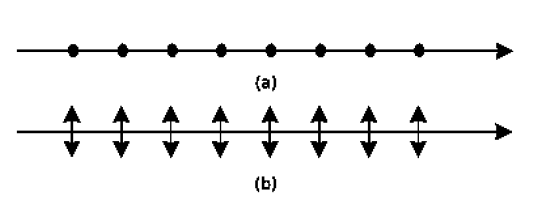
\includegraphics[scale=0.5]{1.png}
	\caption{(a) Linearly polarized light with the polarization axis perpendicular to the page plane. (b) Linearly polarized light with the polarization axis parallel to the page plane.}
\end{figure}
\begin{figure}[H]
	\centering
	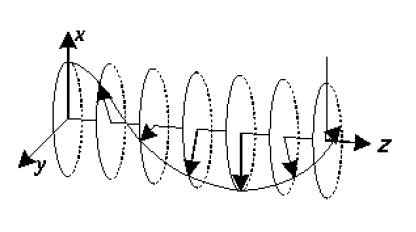
\includegraphics[scale=0.5]{2.png}
	\caption{Elliptically polarized light propagating in the z direction. The light is polarized in the $ xy $ plane.}
\end{figure}

\subsection{Polarizer}
A device commonly used to produce polarized light is a polaroid (also called a po-
larizer). It polarizes the light using the principle of dichroism: a selective absorptio mechanism tends to allow the light polarized in a certain direction (direction of the crystal alignment) to pass through the material, while the light polarized in all other directions is absorbed. This turns the incident natural light into linearly polarized.

A polarization device can not only change incident natural light to polarized light (it then acts as a polarizer), but may also be used to detect and analyze linearly polarized, natural, and partially polarized light (it is then called an analyzer).

\subsection{Malus' law}
A visible effect in the light coming out of a polarization device is a change of the light brightness.

Suppose that we have two polarizers arranged so that their planes are parallel- the left one plays the role of a polarizer, the other one is an analyzer (Figure 3). Let the angle between their transmission directions (polarization axes) be $ \theta $. The light is incident normally on the polarizer and then continues to the analizer. The intensity of the linearly polarized light leaving the analyzer is
\begin{equation}
	I_{light}=I_{light,0}cos^2\theta
\end{equation}
where $ I_{light,0} $ is the intensity of the linearly polarized light incident on the analyzer. Equation (1), named after Etienne-Louis Malus as the Malus' law, was derived in 1809.

Obviously, for a single polarizer, if polarized light is incident on it, then the transmitted light intensity will change periodically when rotating the polarizer. If the incident light is partially or elliptically polarized, the minimum intensity will not be zero as there will be always some component of the light polarized in the transmission direction. The incident light must be natural or circularly polarized if the intensity does not change at all. Hence, by using a polarizer, one can distinguish linearly polarized light from the natural and circularly polarized light.

\begin{figure}[H]
	\centering
	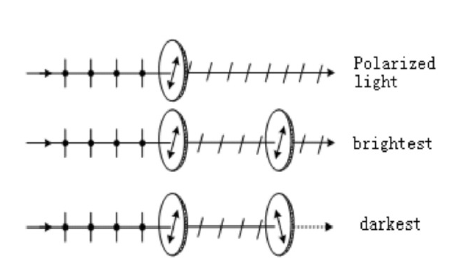
\includegraphics[scale=0.5]{3.png}
	\caption{Change in the brightness of the light depends on the mutual orientation of the polarizer and the analyzer.}
\end{figure}


\subsection{Generation of Elliptically and Circularly Polarized Light.Half-wave and Quarter-wave Plates}
Suppose that a linearly polarized light is incident morally on a crystal plate whose surface is parallel to its optical axis, and the angle between the polarizing axis and the optical axis of the plate is $ \alpha $. Then the linearly polarized light is resolved into two waves: an e-wave with the oscillation direction parallel to the optical axis of the plate (extraordinary axis) and an o-wave whose oscillation direction is perpendicular to the optical axis (ordinary axis). They propagate in the same direction, but with different
speeds. The resulting optical path difference over the thickness d of the plate is
$$ \Delta=(n_e-n_o)d $$
and, consequently, the phase difference
$$ \delta=\dfrac{2\pi}{\lambda}(n_3-n_o)d $$
where $ \lambda $ is the wavelength, ne is the refractive index for the extraordinary axis, and no is the refractive index for the ordinary axis. In a so-called positive crystal $ \delta > 0 $, whereas in a negative one $ \delta < 0 $.
\begin{figure}[H]
	\centering
	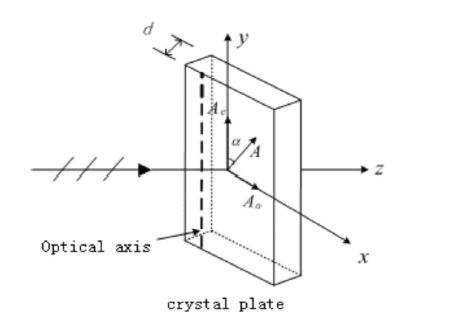
\includegraphics[scale=0.5]{4.png}
	\caption{Linearly polarized light passing through a waveplate.}
\end{figure}
As shown in Figure 4, when the light propagates through the crystal plate, the two
components of the light vector are
$$ E_x=A_ocos\omega t\qquad E_y=A_ecos(\omega t+\delta) $$
where $ A_e=Acos\alpha,A_o=Asin\alpha $. Eliminating time from the above equations one obtains
\begin{equation}
	\dfrac{E_x^2}{A_o^2}+\dfrac{E_y^2}{A_e^2}-2\dfrac{E_xE_y}{A_oA_e}cos\delta=sin^\delta
\end{equation}
which is the equation of an ellipse.
When the thickness of the plate changes, the optical path difference changes as well. Some cases of particular interest, are discussed below:
\begin{enumerate}[$\blacktriangleright$]
	\item If $ \Delta=k\lambda $, where $ k=0,1,2,\cdots, $ the phase difference $ \delta=0 $, and Eq.(2) reduces to 
	$$ E_y=\dfrac{A_e}{A_o}E_x $$
	which is a linear equation. Hence the transmitted light is linearly polarized with the oscillation direction remaining unchanged. A waveplate that satisfies this condition is called a full-wave plate. The light goes through a full-wave plate without changing its polarization state.
	\item If $ \Delta=(2k+1)\lambda/2 $, where $ k=0,1,2,\cdots $, the phase difference $ \delta=\pi $, and Eq. (2) simplifies to 
	$$ E_y=-\dfrac{A_e}{A_o}E_x $$
	The transmitted light is also linearly polarized with the polarization axis rotated by the angle of $ 2\alpha $. A waveplate that satisfies the condition is called 1/2-wave plate or half-wave plate. When a polarized light passes through a half-wave plate, its polarization axis gets rotated by an angle $ 2\alpha $. If $ \alpha=\pi/4 $, then the polarization axis of the transmitted light is perpendicular to that of the incident light.
	\item Finally, if $ \Delta=(2k+1)\lambda/4 $, where $ k=0,1,2,\cdots $, the phase difference $ \delta=\pm\pi/2 $. and Eq.(2) transforms into
	$$  \dfrac{E_x^2}{A_o^2}\pm\dfrac{E_y^2}{A_e^2}=1 $$
	The transmitted light is elliptically polarized withA waveplate that satisfies the above condition is called a 1/4-wave plate or a quarter-waveplate and is an important optical element in many polarization experiments.
\end{enumerate}
If $ A_e = A_o = A $, then $ E^2_x + E^2_y = A^2 $, and the transmitted light is circularly polarized. Since the amplitudes of the o-wave and the e-wave are both functions of $ \alpha $, the polarization state after passing through a 1/4-wave plate will vary, depending on the angle:
\begin{enumerate}[$\blacktriangleright$]
	\item if $ \alpha= 0 $, the transmitted light is linearly polarized with the polarization axis parallel to the optical axis of the 1/4-wave plate;
	\item if $ \alpha=\pi/2 $, the transmitted light is linearly polarized with the polarization axis perpendicular to the optical axis of the 1/4-wave plate;
	\item if $ \alpha=\pi/4 $,the transmitted light is circularly polarized;
	\item otherwise, the transmitted light is elliptically polarized.
\end{enumerate}
\section{Measurement Setup and Procedure}
\subsection{Apparatus}
The main elements of the measurement setup are: a semiconductor laser, a tungsten
iodine lamp, a silicon photo-cell, a UT51 digital universal meter, two polarizers, a 1/2- wave plate, a 1/4-wave plate, a reflector and a stack of glass. The elements are placed on an optical bench.

\subsection{Measurement Procedure and Data Analysis}
\subsubsection{Demonstration of Malus' Law}
\begin{enumerate}
	\item Assemble the measurement setup as shown in Figure 5. Make sure that the laser ray passes through the polarizer to generate linearly polarized light before continuing to the analyzer and the silicon photo-cell.
	\item Rotate the analyzer for $ 360^\circ $ and observe a change in the light intensity to find the maximum electric current $ I_0 $.
	\item Set the angle of analyzer to $ 90^\circ $ and adjust the angle of the polarizer until the electric current measured by the multimeter reaches its minimum. At this point, the polarizing axes of the polarizer and the analyzer are perpendicular to each other.
	\item Rotate the analyzer from $ 90^\circ $ to $ 0^\circ $ and record the magnitude of the current $ I $ every $ 5^\circ $. Record the values in a table and plot the graph $ I/I_0 $ vs. $ cos^2\theta $. Perform linear fitting and compare the data with the theoretical result.
\end{enumerate}
\begin{figure}[H]
	\centering
	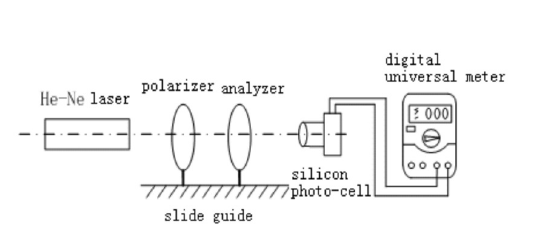
\includegraphics[scale=0.5]{5.png}
	\caption{Experimental setup for a demonstration of Malus' law.}
\end{figure}
\subsubsection{Linearly Polarized Light and the Half-wave Plate}
\begin{enumerate}
	\item Set up the equipment on the optical bench as shown in Figure 6. A is the analyzer and P is the polarizer. Set the polarizing axes of A and P perpendicular to each other before placing the 1/2-wave plate in the apparatus; extinction of the light can be observed on screen.
	\item After inserting the 1/2-wave plate, rotate it to make the light extinction appear again and set this position as the initial position.
	\item Rotate the 1/2-wave plate for $ \alpha= 10^\circ $ from the initial position and the light extinction will be broken. Then rotate A to make the light extinction appear again, record the angle of rotation $ \Delta \theta  $ in a table.
	\item Rotate the 1/2-wave plate for $ 10^\circ $ from the previous position (now $ \alpha=2^\circ $) and repeat Step 3. Repeat this step (increase $ \alpha $) for 8 times. Plot the graph $ \Delta\theta $ vs. $\theta. $
	\item After analyzing the data, the following questions will be answered:
	\begin{enumerate}
		\item How many times can the light extinction be observed when the 1/2-wave plate rotates for $ 360^\circ $?
		\item How many times can the light extinction be observed when the analyzer rotates for $ 360^\circ $?
		\item Explain the polarization state of linearly polarized light after passing through the 1/2-wave plate.
	\end{enumerate}
\end{enumerate}
\begin{figure}[H]
	\centering
	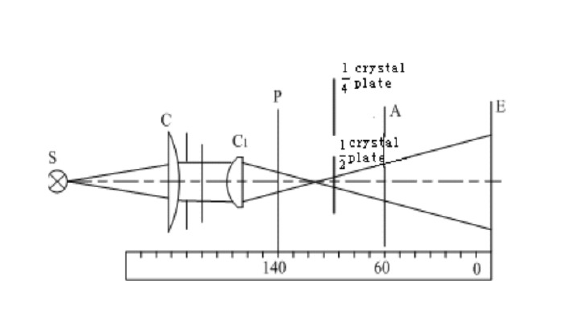
\includegraphics[scale=0.5]{6.png}
	\caption{Experimental setup for the 1/2-wave plate.}
\end{figure}

\subsubsection{Circularly and Elliptically Polarized Light and the 1/4-wave Plate}
\begin{enumerate}
	\item Set up the equipment on the optical bench as shown in Figure 6. A is the analyzer and P is the polarizer. Set the polarizing axes of A and P perpendicular to each other before placing the 1/4-wave plate in the apparatus; extinction of the light can be observed on screen. At this point the angle $ \theta=90^\circ. $
	\item After inserting the 1/4-wave plate, rotate it to make the light extinction appear again and set this position as the initial position. At this point $ \alpha=0^\circ $. Rotate the 1/4-wave plate and observe the change in the light intensity.
	\item Rotate the analyzer for $ 360^\circ $ and record the light intensity (which is indicated by the current $ I $) for every $ 10^\circ $. Record the data in a table.
	\item Rotate the 1/4-wave plate for $ 20^\circ $, repeat Step 3.
	\item Rotate the 1/4-wave plate for $ 45^\circ $, repeat Step 3.
	\item Rotate the 1/4-wave plate for $ 70^\circ $. Then rotate the analyzer and record its position	and the magnitude of the current when the light intensity reaches a maximum.
	\item Use a computer to plot the relation between the rotation angle of the analyzer and the light amplitude in polar coordinates. Normalize the amplitude by its maximum value. Mark the position recorded in Step 6 and compare it with the data recorded in Step 4.
	
	Pay attention to the fact that the light intensity is found indirectly by measuring the electric current, and the intensity is proportional to the amplitude squared. The current indicates the intensity, not the amplitude.
	\item Compare the result of Step 5 with that for the circular polarization. Plot a linear fit to the data when the angle is $ 45^\circ $.
\end{enumerate}

\newpage

\section{Results}

Uncertainty of $\theta$ is [2$^\circ$]

\subsection{Demonstration of Malus' Law}

The measurement of current $I$ was shown in Table \ref{tab-1}.

\begin{table}[!h]
\begin{center}
\begin{tabular}{|c|c||c|c|}
\hline
\multicolumn{4}{|c|}{Maximum Electric Current $I_0$ $6.852\pm0.001$ [$\mu A$]}\\
\hline
$\theta$&$I[\mu A]\pm0.01[\mu A]$&$\theta$&$I[\mu A]\pm0.01[\mu A]$\\
\hline
$0^\circ$	&	6.728	&	$50^\circ$	&	2.781	\\
\hline
$5^\circ$	&	6.667	&	$55^\circ$	&	2.227	\\
\hline
$10^\circ$	&	6.519	&	$60^\circ$	&	1.697	\\
\hline
$15^\circ$	&	6.303	&	$65^\circ$	&	1.141	\\
\hline
$20^\circ$	&	5.966	&	$70^\circ$	&	0.708	\\
\hline
$25^\circ$	&	5.542	&	$75^\circ$	&	0.399	\\
\hline
$30^\circ$	&	5.078	&	$80^\circ$	&	0.136	\\
\hline
$35^\circ$	&	4.536	&	$85^\circ$	&	-0.012	\\
\hline
$40^\circ$	&	3.989	&	$90^\circ$	&	-0.063	\\
\hline
$45^\circ$	&	3.343	&				&			\\
\hline
\end{tabular}
\caption{Measurement data Malus's law demonstration.}
\label{tab-1}
\end{center}
\end{table}

The fitted curve was plotted in Figure \ref{fig-1}.\\

\begin{figure}[H]
\centering
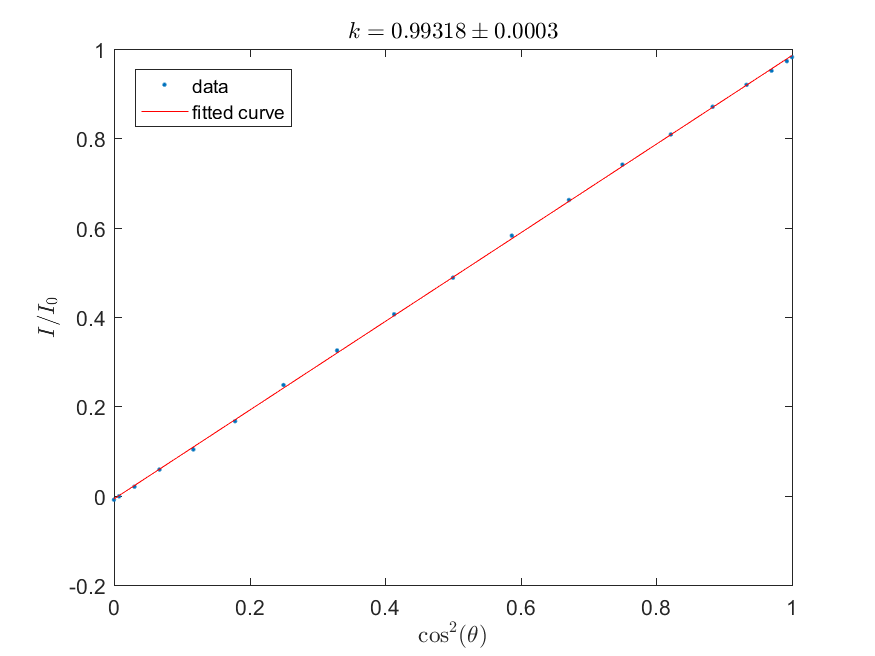
\includegraphics[scale=0.5]{fig1.png}
\caption{Fit graph for Table \ref{tab-1}.}
\label{fig-1}
\end{figure}

\newpage

\subsection{Linearly Polarized Light and the Half-wave Plate}

The measurement data for the 1/2-wave plate was shown in Table \ref{tab-2}.

\begin{table}[!h]
\begin{center}
\begin{tabular}{|c|c|}
\hline
Rotating angle of the 1/2-wave plate&Rotation angle of the analyzer $[^\circ]\pm2[^\circ]$\\
\hline
initial		&	$0^\circ$	\\
\hline
$10^\circ$	&	$20^\circ$	\\
\hline
$20^\circ$	&	$40^\circ$	\\
\hline
$30^\circ$	&	$60^\circ$	\\
\hline
$40^\circ$	&	$80^\circ$	\\
\hline
$50^\circ$	&	$100^\circ$	\\
\hline
$60^\circ$	&	$118^\circ$	\\
\hline
$70^\circ$	&	$138^\circ$	\\
\hline
$80^\circ$	&	$156^\circ$	\\
\hline
$90^\circ$	&	$174^\circ$	\\
\hline
\end{tabular}
\caption{Measurement data for the 1/2-wave plate.}
\label{tab-2}
\end{center}
\end{table}

The fitted curve was plotted in Figure \ref{fig-2}.\\

\begin{figure}[H]
\centering
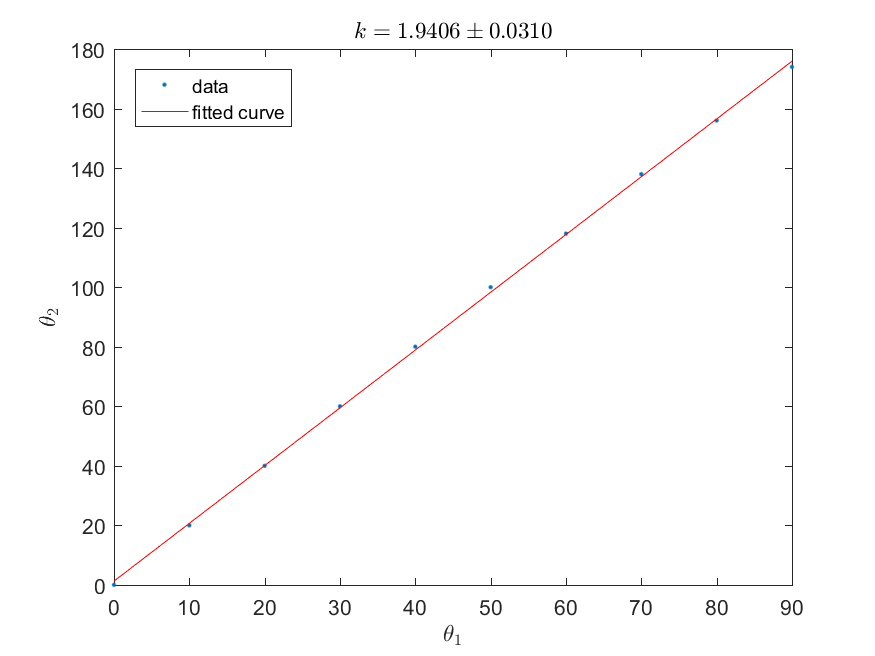
\includegraphics[scale=0.5]{fig2.png}
\caption{Fit graph for Table \ref{tab-2}.}
\label{fig-2}
\end{figure}

When the 1/2-wave plate rotates for $360^\circ$, 4 light extinctions can be observed.\\

When the analyzer rotates for $360^\circ$, 2 light extinctions can be observed.\\

When the 1/2-wave plate rotates for $\theta$, the analyzer rotates for $2\theta$.\\

\newpage


\subsection{Circularly and Elliptically Polarized Light and the 1/4-wave Plate}

The measurement of current $I$ was shown in Table \ref{tab-deg-0}.
\begin{table}[!h]
\begin{center}
\begin{tabular}{|c|c|c||c|c|c|}
\hline
\multicolumn{6}{|c|}{Rotation angle of 1/4-wave plate: $0^\circ$}\\
\hline
\multicolumn{6}{|c|}{Maximum Electric Current $I_0$ $4.785\pm0.001$ [$\mu A$]}\\
\hline
$\theta$&$I[\mu A]\pm0.01[\mu A]$&$I/I_0$&$\theta$&$I[\mu A]\pm0.01[\mu A]$&$I/I_0$\\
\hline
$0^\circ$	&	4.771	&	$0.997\pm0.0003$	&	$180^\circ$	&	4.781	&	$0.999\pm0.0003$	\\
\hline
$10^\circ$	&	4.651	&	$0.972\pm0.0003$	&	$190^\circ$	&	4.677	&	$0.977\pm0.0003$	\\
\hline
$20^\circ$	&	4.261	&	$0.890\pm0.0003$	&	$200^\circ$	&	4.300	&	$0.899\pm0.0003$	\\
\hline
$30^\circ$	&	3.660	&	$0.765\pm0.0003$	&	$210^\circ$	&	3.725	&	$0.778\pm0.0003$	\\
\hline
$40^\circ$	&	2.870	&	$0.600\pm0.0002$	&	$220^\circ$	&	2.955	&	$0.618\pm0.0002$	\\
\hline
$50^\circ$	&	2.053	&	$0.429\pm0.0002$	&	$230^\circ$	&	2.112	&	$0.441\pm0.0002$	\\
\hline
$60^\circ$	&	1.246	&	$0.260\pm0.0002$	&	$240^\circ$	&	1.300	&	$0.272\pm0.0002$	\\
\hline
$70^\circ$	&	0.617	&	$0.129\pm0.0002$	&	$250^\circ$	&	0.635	&	$0.133\pm0.0002$	\\
\hline
$80^\circ$	&	0.153	&	$0.032\pm0.0002$	&	$260^\circ$	&	0.179	&	$0.037\pm0.0002$	\\
\hline
$90^\circ$	&	0.001	&	$0.000\pm0.0002$	&	$270^\circ$	&	0.000	&	$0.000\pm0.0002$	\\
\hline
$100^\circ$	&	0.089	&	$0.019\pm0.0002$	&	$280^\circ$	&	0.103	&	$0.022\pm0.0002$	\\
\hline
$110^\circ$	&	0.468	&	$0.098\pm0.0002$	&	$290^\circ$	&	0.479	&	$0.100\pm0.0002$	\\
\hline
$120^\circ$	&	1.065	&	$0.223\pm0.0002$	&	$300^\circ$	&	1.094	&	$0.229\pm0.0002$	\\
\hline
$130^\circ$	&	1.820	&	$0.380\pm0.0002$	&	$310^\circ$	&	1.863	&	$0.389\pm0.0002$	\\
\hline
$140^\circ$	&	2.656	&	$0.555\pm0.0002$	&	$320^\circ$	&	2.737	&	$0.572\pm0.0002$	\\
\hline
$150^\circ$	&	3.475	&	$0.726\pm0.0003$	&	$330^\circ$	&	3.498	&	$0.731\pm0.0003$	\\
\hline
$160^\circ$	&	4.157	&	$0.869\pm0.0003$	&	$340^\circ$	&	4.159	&	$0.869\pm0.0003$	\\
\hline
$170^\circ$	&	4.601	&	$0.962\pm0.0003$	&	$350^\circ$	&	4.615	&	$0.964\pm0.0003$	\\
\hline
\end{tabular}
\caption{Measurement data for the 1/4-wave plate (rotation angle $0^\circ$).}\label{tab-deg-0}
\end{center}
\end{table}

The relation between rotation angle and light intensity was plotted in Figure \ref{fig-deg-0}.
\begin{figure}[H]
\centering
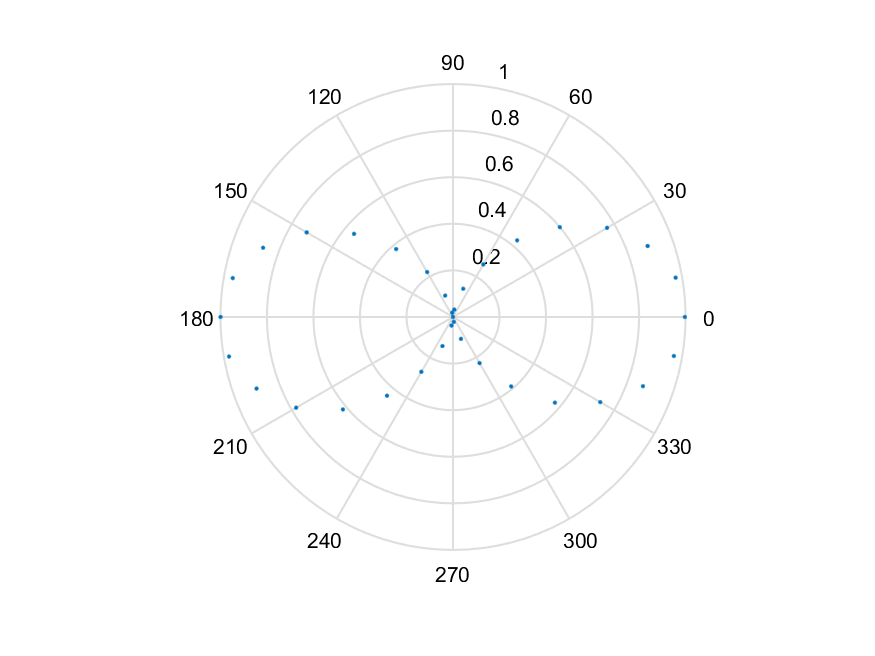
\includegraphics[scale=0.5]{deg-0.png}
\caption{$\theta$ vs. $I/I_0$ graph.}
\label{fig-deg-0}
\end{figure}



\newpage
The measurement of current $I$ was shown in Table \ref{tab-deg-20}.
\begin{table}[!h]
\begin{center}
\begin{tabular}{|c|c|c||c|c|c|}
\hline
\multicolumn{6}{|c|}{Rotation angle of 1/4-wave plate: $20^\circ$}\\
\hline
\multicolumn{6}{|c|}{Maximum Electric Current $I_0$ $4.169\pm0.001$ [$\mu A$]}\\
\hline
$\theta$&$I[\mu A]\pm0.01[\mu A]$&$I/I_0$&$\theta$&$I[\mu A]\pm0.01[\mu A]$&$I/I_0$\\
\hline
$0^\circ$	&	3.641	&	$0.873\pm0.0003$	&	$180^\circ$	&	3.637	&	$0.872\pm0.0003$	\\
\hline
$10^\circ$	&	4.010	&	$0.962\pm0.0003$	&	$190^\circ$	&	4.001	&	$0.960\pm0.0003$	\\
\hline
$20^\circ$	&	4.163	&	$0.999\pm0.0003$	&	$200^\circ$	&	4.169	&	$1.000\pm0.0003$	\\
\hline
$30^\circ$	&	4.087	&	$0.980\pm0.0003$	&	$210^\circ$	&	4.103	&	$0.984\pm0.0003$	\\
\hline
$40^\circ$	&	3.797	&	$0.911\pm0.0003$	&	$220^\circ$	&	3.827	&	$0.918\pm0.0003$	\\
\hline
$50^\circ$	&	3.313	&	$0.795\pm0.0003$	&	$230^\circ$	&	3.551	&	$0.852\pm0.0003$	\\
\hline
$60^\circ$	&	2.700	&	$0.648\pm0.0003$	&	$240^\circ$	&	2.765	&	$0.663\pm0.0003$	\\
\hline
$70^\circ$	&	2.056	&	$0.493\pm0.0003$	&	$250^\circ$	&	2.108	&	$0.506\pm0.0003$	\\
\hline
$80^\circ$	&	1.433	&	$0.344\pm0.0003$	&	$260^\circ$	&	1.478	&	$0.355\pm0.0003$	\\
\hline
$90^\circ$	&	0.981	&	$0.235\pm0.0002$	&	$270^\circ$	&	0.953	&	$0.229\pm0.0002$	\\
\hline
$100^\circ$	&	0.626	&	$0.150\pm0.0002$	&	$280^\circ$	&	0.604	&	$0.145\pm0.0002$	\\
\hline
$110^\circ$	&	0.461	&	$0.111\pm0.0002$	&	$290^\circ$	&	0.452	&	$0.108\pm0.0002$	\\
\hline
$120^\circ$	&	0.518	&	$0.124\pm0.0002$	&	$300^\circ$	&	0.518	&	$0.124\pm0.0002$	\\
\hline
$130^\circ$	&	0.791	&	$0.190\pm0.0002$	&	$310^\circ$	&	0.801	&	$0.192\pm0.0002$	\\
\hline
$140^\circ$	&	1.261	&	$0.302\pm0.0003$	&	$320^\circ$	&	1.292	&	$0.310\pm0.0003$	\\
\hline
$150^\circ$	&	1.828	&	$0.438\pm0.0003$	&	$330^\circ$	&	1.854	&	$0.445\pm0.0003$	\\
\hline
$160^\circ$	&	2.482	&	$0.595\pm0.0003$	&	$340^\circ$	&	2.550	&	$0.612\pm0.0003$	\\
\hline
$170^\circ$	&	3.117	&	$0.748\pm0.0003$	&	$350^\circ$	&	3.142	&	$0.754\pm0.0003$	\\
\hline
\end{tabular}
\caption{Measurement data for the 1/4-wave plate (rotation angle $20^\circ$).}\label{tab-deg-20}
\end{center}
\end{table}

The relation between rotation angle and light intensity was plotted in Figure \ref{fig-deg-20}.
\begin{figure}[H]
\centering
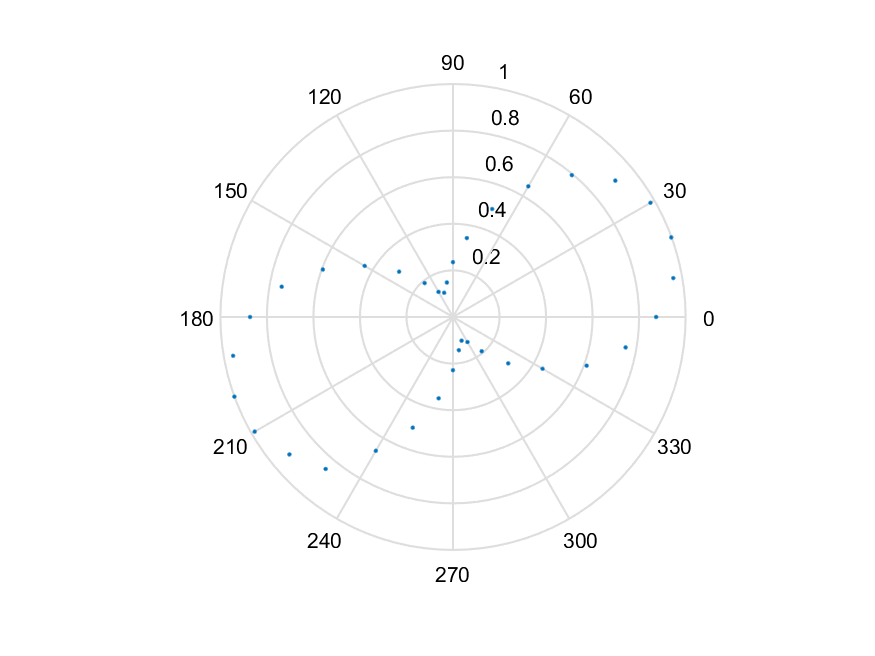
\includegraphics[scale=0.5]{deg-20.png}
\caption{$\theta$ vs. $I/I_0$ graph.}
\label{fig-deg-20}
\end{figure}



\newpage
The measurement of current $I$ was shown in Table \ref{tab-deg-45}.
\begin{table}[!h]
\begin{center}
\begin{tabular}{|c|c|c||c|c|c|}
\hline
\multicolumn{6}{|c|}{Rotation angle of 1/4-wave plate: $45^\circ$}\\
\hline
\multicolumn{6}{|c|}{Maximum Electric Current $I_0$ $2.452\pm0.001$ [$\mu A$]}\\
\hline
$\theta$&$I[\mu A]\pm0.01[\mu A]$&$I/I_0$&$\theta$&$I[\mu A]\pm0.01[\mu A]$&$I/I_0$\\
\hline
$0^\circ$	&	2.350	&	$0.958\pm0.0006$	&	$180^\circ$	&	2.349	&	$0.958\pm0.0006$	\\
\hline
$10^\circ$	&	2.388	&	$0.974\pm0.0006$	&	$190^\circ$	&	2.390	&	$0.975\pm0.0006$	\\
\hline
$20^\circ$	&	2.421	&	$0.987\pm0.0006$	&	$200^\circ$	&	2.431	&	$0.991\pm0.0006$	\\
\hline
$30^\circ$	&	2.441	&	$0.996\pm0.0006$	&	$210^\circ$	&	2.444	&	$0.997\pm0.0006$	\\
\hline
$40^\circ$	&	2.446	&	$0.998\pm0.0006$	&	$220^\circ$	&	2.451	&	$1.000\pm0.0006$	\\
\hline
$50^\circ$	&	2.434	&	$0.993\pm0.0006$	&	$230^\circ$	&	2.441	&	$0.996\pm0.0006$	\\
\hline
$60^\circ$	&	2.410	&	$0.983\pm0.0006$	&	$240^\circ$	&	2.420	&	$0.987\pm0.0006$	\\
\hline
$70^\circ$	&	2.373	&	$0.968\pm0.0006$	&	$250^\circ$	&	2.382	&	$0.971\pm0.0006$	\\
\hline
$80^\circ$	&	2.333	&	$0.951\pm0.0006$	&	$260^\circ$	&	2.333	&	$0.951\pm0.0006$	\\
\hline
$90^\circ$	&	2.297	&	$0.937\pm0.0006$	&	$270^\circ$	&	2.295	&	$0.936\pm0.0006$	\\
\hline
$100^\circ$	&	2.255	&	$0.920\pm0.0006$	&	$280^\circ$	&	2.251	&	$0.918\pm0.0006$	\\
\hline
$110^\circ$	&	2.224	&	$0.907\pm0.0006$	&	$290^\circ$	&	2.222	&	$0.906\pm0.0006$	\\
\hline
$120^\circ$	&	2.211	&	$0.902\pm0.0005$	&	$300^\circ$	&	2.199	&	$0.897\pm0.0005$	\\
\hline
$130^\circ$	&	2.206	&	$0.900\pm0.0005$	&	$310^\circ$	&	2.192	&	$0.894\pm0.0005$	\\
\hline
$140^\circ$	&	2.214	&	$0.903\pm0.0005$	&	$320^\circ$	&	2.204	&	$0.899\pm0.0005$	\\
\hline
$150^\circ$	&	2.237	&	$0.912\pm0.0006$	&	$330^\circ$	&	2.232	&	$0.910\pm0.0006$	\\
\hline
$160^\circ$	&	2.267	&	$0.925\pm0.0006$	&	$340^\circ$	&	2.267	&	$0.925\pm0.0006$	\\
\hline
$170^\circ$	&	2.313	&	$0.943\pm0.0006$	&	$350^\circ$	&	2.303	&	$0.939\pm0.0006$	\\
\hline
\end{tabular}
\caption{Measurement data for the 1/4-wave plate (rotation angle $45^\circ$).}\label{tab-deg-45}
\end{center}
\end{table}

The relation between rotation angle and light intensity was plotted in Figure \ref{fig-deg-45}.
\begin{figure}[H]
\centering
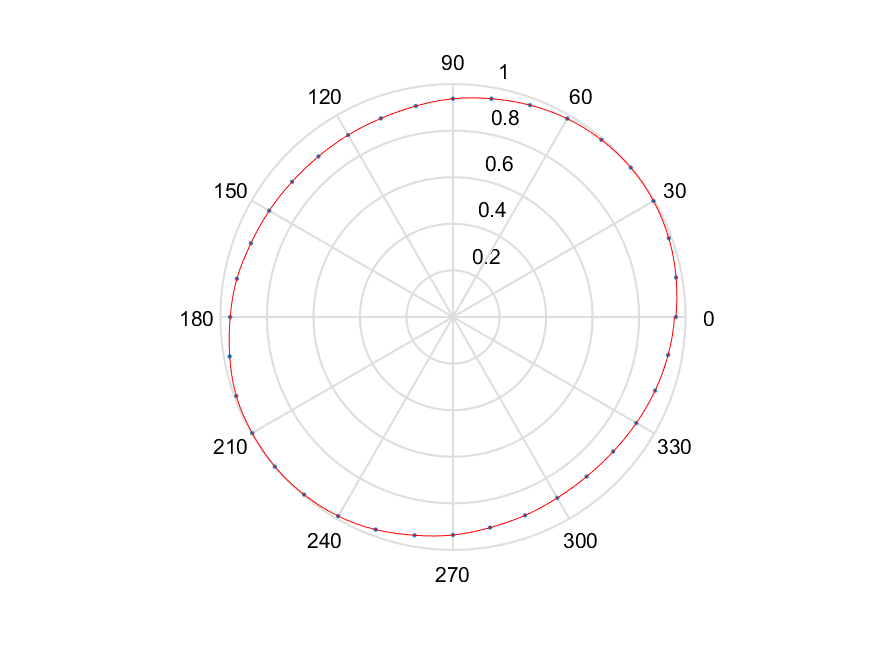
\includegraphics[scale=0.5]{deg-45.png}
\caption{$\theta$ vs. $I/I_0$ graph.}
\label{fig-deg-45}
\end{figure}


\newpage

The measurement of current $I$ was shown in Table \ref{tab-6}.
\begin{table}[!h]
\begin{center}
\begin{tabular}{|c|c|}
\hline
\multicolumn{2}{|c|}{Rotating angle of the 1/2-wave plate: $70^\circ$}\\
\hline
$\theta[^\circ]\pm2[^\circ]$		&	$161^\circ$	\\
\hline
$I[\mu A]\pm0.01[\mu A]$	&	4.114	\\
\hline
\end{tabular}
\caption{Measurement data for the 1/2-wave plate (rotation angle $70^\circ$).}
\label{tab-6}
\end{center}
\end{table}

The maximum $I$ when the angle is $20^\circ$, $\theta_1\approx180^\circ$\\

The maximum $I$ when the angle is $70^\circ$, $\theta_1\approx161^\circ$\\
$$\theta_1+\theta_2=341^\circ$$

which proves that the theorem is true.

\section{Measurement uncertainty analysis}

The uncertainty of $\cos^2\theta$ can be  found by applying the uncertainty propagation formula

\begin{align*}
u_{\cos^2\theta}=2sin\theta\cos\theta u_{\theta}
\end{align*}

The uncertainty of $I/I_0$ can be found by applying the uncertainty propagation formula

\begin{align*}
u_{I/I_0}&=\sqrt{\left(\frac{\partial I/I_0}{\partial I}\right)^2u_{I}^2+\left(\frac{\partial I/I_0}{\partial I_0}\right)^2u_{I_0}^2}\\
&=\sqrt{\left(\frac{1}{I_0}\right)^2u_{I}^2+\left(\frac{I}{I_0^2}\right)^2u_{I_0}^2}\\
\end{align*}


\section{Conclusion}

In this lab, we understand some properties of light, in particular to study the polarization phenomenon and verify Malus' law, the way half- and quarter-wave plates work in optical systems and generation and detection of elliptically and circularly polarized light.\\

A visible effect in the light coming out of a polarization device is a change of the light brightness.

$$I_{light}=I_{light,0}cos^2\theta$$

Since the amplitudes of the o-wave and the e-wave are both functions of $ \alpha $, the polarization state after passing through a 1/4-wave plate will vary, depending on the angle:\\

If $ \alpha= 0 $, the transmitted light is linearly polarized with the polarization axis parallel to the optical axis of the 1/4-wave plate;

If $ \alpha=\pi/2 $, the transmitted light is linearly polarized with the polarization axis perpendicular to the optical axis of the 1/4-wave plate;

If $ \alpha=\pi/4 $,the transmitted light is circularly polarized;

Otherwise, the transmitted light is elliptically polarized.


\section{Reference}

\begin{enumerate}[(a)]
	\item
	Qin Tian, Cao Jianjun, Mateusz Krzyzosiak, VP241 Exercise 3, Polarization of Light, based on materials provided by the Department of Physics, Shanghai Jiaotong University.
\end{enumerate}

\section{Data sheet}

The Data sheet is attached at the end of the report.

\end{document}
